\documentclass[a4paper,11pt]{article}
%Przydatne paczki:
\usepackage{amssymb}
\usepackage{amsthm}
\usepackage{amsmath}
\usepackage[colorinlistoftodos]{todonotes}
\usepackage[colorlinks=true, allcolors=blue]{hyperref}
%Definicja kodowania i języka:
\usepackage[polish]{babel}
\usepackage[MeX]{polski}
\usepackage[utf8]{inputenc}
\usepackage[T1]{fontenc}
%Paczki dodane w drodze pisania:
\usepackage{graphicx}
\usepackage{anysize}
\selectlanguage{polish}
\usepackage{tabularx}
\usepackage[export]{adjustbox}
\usepackage{listings}
\usepackage{float}
\usepackage{fancyhdr}
\usepackage{listing}

%Nagłówek:
\pagestyle{fancy}
\fancyhead{}
\fancyhead[L]{\small{\bfseries \thepage}}
\fancyfoot[L, C, R] {}
\fancyhead[C]{\small{\bfseries Dokumentacja projektu "Reflekto"}}
\renewcommand{\headrulewidth}{0.8pt}

%\marginsize{left}{right}{top}{bottom}
\marginsize{2.5cm}{2.5cm}{2.5cm}{2.5cm}
\lstdefinelanguage{C}{
	keywords={typeof, new, true, false, catch, function, return, null, catch, switch, var, if, in, while, do, else, case, break},
	keywordstyle=\color{blue}\bfseries,
	ndkeywords={class, export, boolean, throw, implements, import, this},
	ndkeywordstyle=\color{darkgray}\bfseries,
	identifierstyle=\color{black},
	sensitive=false,
	comment=[l]{//},
	morecomment=[s]{/*}{*/},
	commentstyle=\color{purple}\ttfamily,
	stringstyle=\color{red}\ttfamily,
	morestring=[b]',
	morestring=[b]"
}

\lstset{
	language=C,
	backgroundcolor=\color{lightgray},
	extendedchars=true,
	basicstyle=\footnotesize\ttfamily,
	showstringspaces=false,
	showspaces=false,
	numbers=left,
	numberstyle=\footnotesize,
	numbersep=9pt,
	tabsize=2,
	breaklines=true,
	showtabs=false,
	captionpos=b
}

\begin{document}

\title{Dokumentacja projektu \\ \textbf{,,Reflekto'' } }
\author{Michał Kwiecień \\ Michał Wójcik}
%skomentować żeby nie było daty
%\date{\vspace{-5ex}}
\maketitle

\begin{abstract}
Dokumentacja projektu inteligentnego lustra w konwencji IoT komunikującego się ze smartfonem z użyciem interfejsu Bluetooth Low Energy. Projekt powstał na potrzeby konkursu Nordic Semiconductor Student Contest. 
\end{abstract}

\begin{figure}
	
\includegraphics[width=0.3\textwidth,center]{logo_nordic.png}
\end{figure}

\cleardoublepage
\tableofcontents
\clearpage

\section{Ogólny opis projektu}

Założeniem projektu jest stworzenie inteligentnego lustra, które podczas wykonywania codziennych czynności umożliwi podgląd najświeższych i spersonalizowanych informacji. Informacje te zostaną wyświetlone na wyświetlaczu umieszczonym za lustrem weneckim, dzięki czemu będą widoczne jednocześnie obok odbicia. 

Działanie lustra opiera się na przekazaniu danych poprzez moduł Bluetooth ze smartfona do modułu nRF52 i umieszczeniu ich na podłączonym ekranie. Aktywacja lustra nastąpi w momencie zbliżenia się do niego użytkownika. Z lustra może korzystać wielu użytkowników, gdyż każdorazowo przesyłane są indywidualne dane dla każdego z nich. 

W celu wygenerowania danych stworzona została dedykowana aplikacja dla systemu iOS. Po wstępnej konfiguracji umożliwi ona zautomatyzowanie procesu i przesyłanie wiadomości w tle bez późniejszych ingerencji użytkownika.


\section{Prezentacja działania}

Kiedy lustro nie jest w bliskim zasięgu jednego ze sparowanych telefonów, wyświetlana jest godzina lub pozostaje ono wyłączone w zależności od ustawień (Rys. \ref{lustro_off})

\begin{figure}[H]
	
\includegraphics[width=0.6\textwidth,center]{mirror_off.png}
	\caption {Lustro w stanie wyłączonym}
	\label{lustro_off}
\end{figure}

W momencie zbliżenia się użytkownika następuje transmisja danych i wyświetlenie aktualnych informacji (Rys. \ref{lustro_on}).

\begin{figure}[H]
	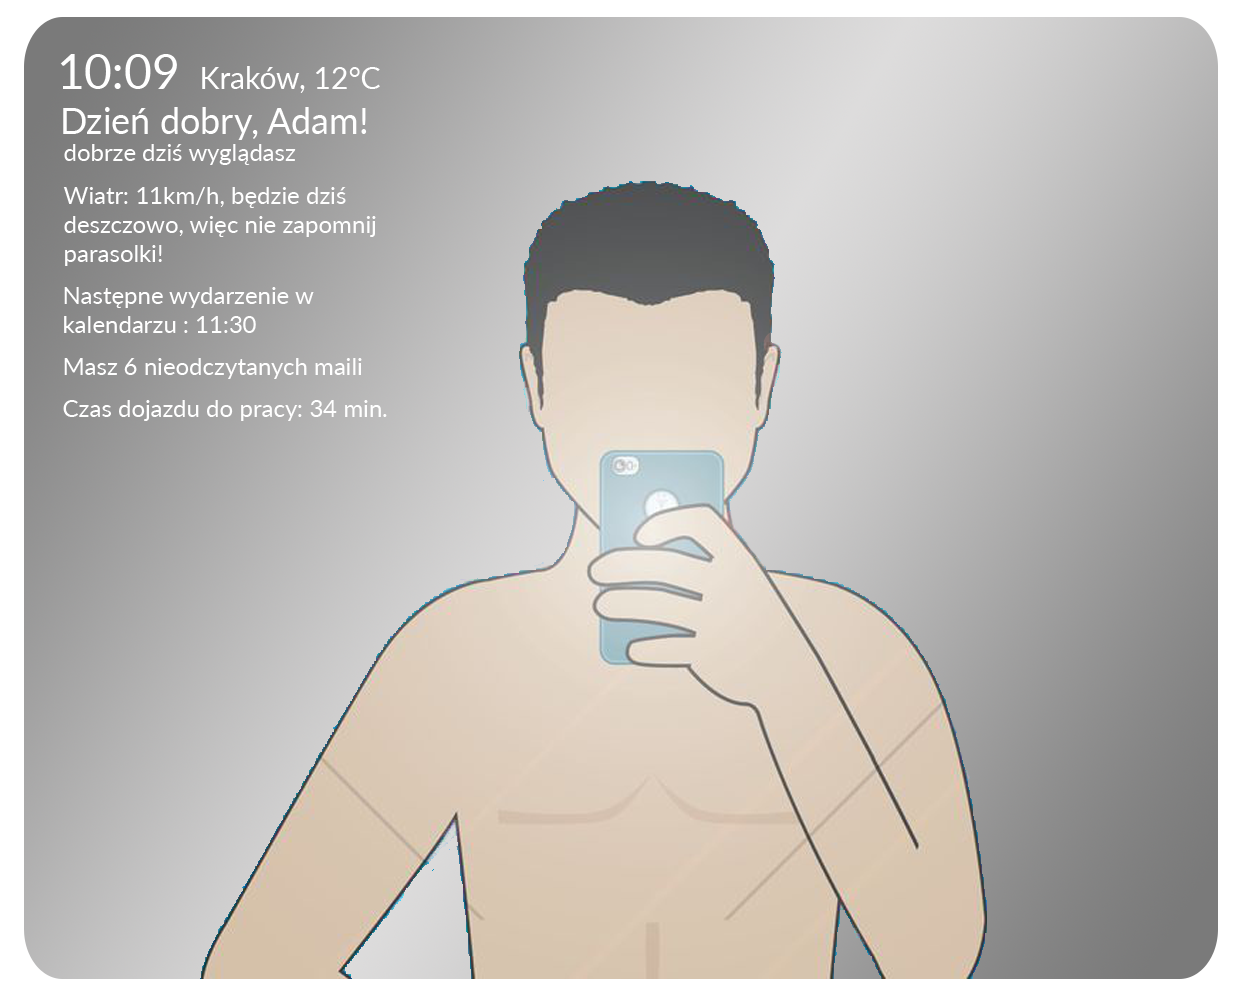
\includegraphics[width=0.6\textwidth,center]{mirror_on.png}
	\caption {Poglądowy rysunek lustra w stanie aktywnym}
	\label{lustro_on}
\end{figure}

\section{Możliwości personalizacji}
\begin{figure}[H]
	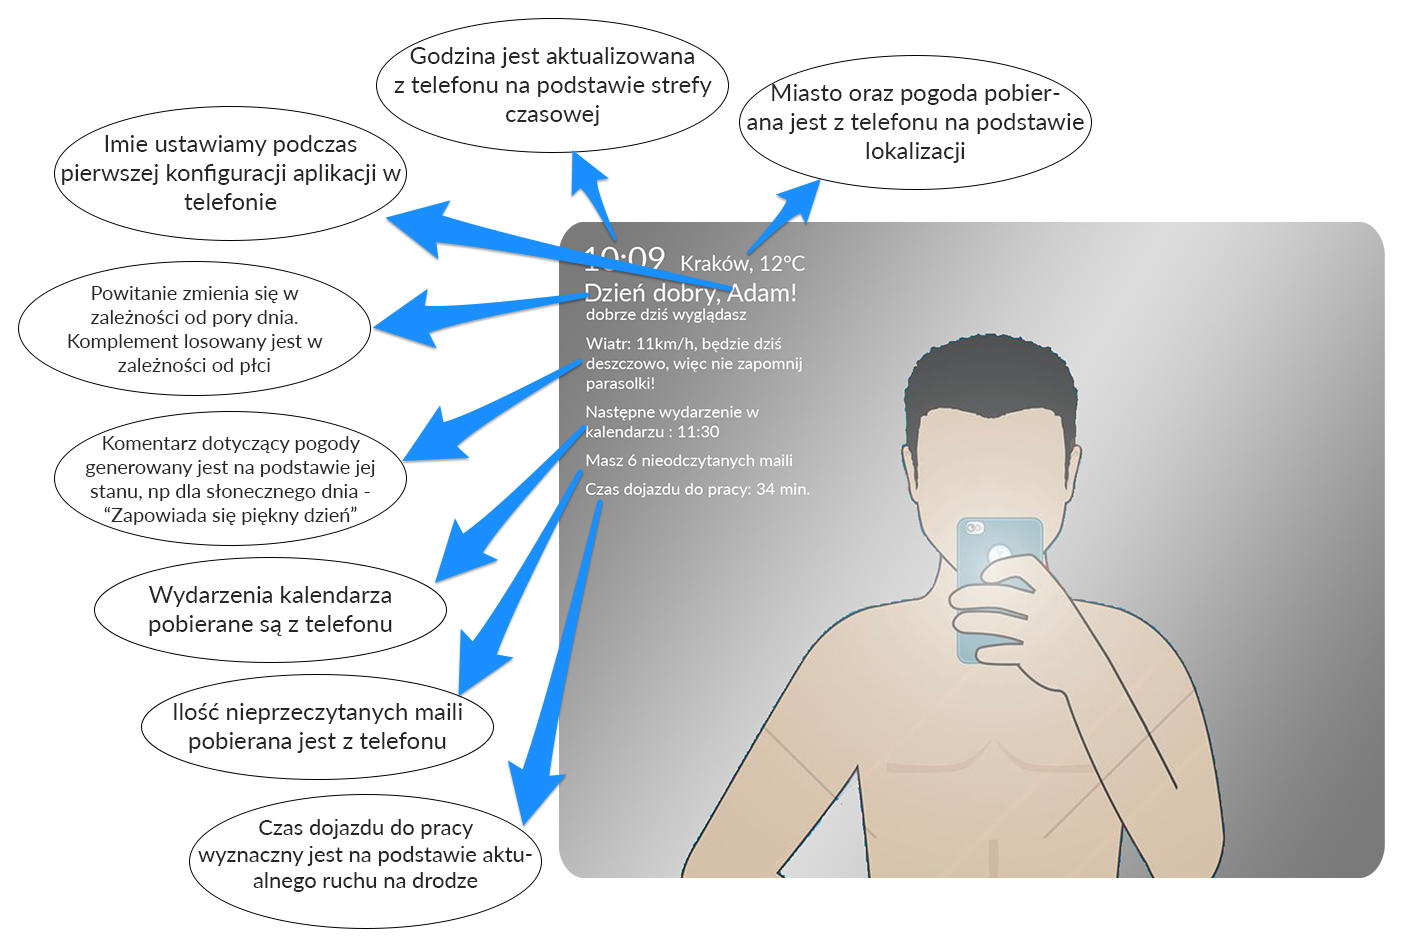
\includegraphics[width=0.9\textwidth,center]{dymki_kreski.png}
	\caption {Poglądowy rysunek możliwości personalizacji}
	\label{lustro_konf}
\end{figure}

\section{Opis aplikacji systemu wbudowanego nRF52}
\subsection{Włączenie urządzenia}
Urządzenie po uruchomieniu inicjalizuje wszystkie niezbędne usługi: timery, stos BLE, serwisy oraz obsługę wyświetlacza. Dalej rozpoczyna się rozgłaszanie (pod nazwą ,,nRF\_Reflekto'') i urządzenie pozostaje w stanie oczekiwania aż do wyłączenia zasilania. 

\subsection{Zasilanie}
Ze względu na użycie wyświetlacza TFT, wymagane jest zasilanie przez zasilacz zewnętrzny bądź port USB (bateria pastylkowa nie pokrywa zapotrzebowania na prąd). Szacowany pobór energii w stanie aktywnym wynosi 400mW. W stanie nieaktywnym pobór energii przez wyświetlacz może zostać zredukowany do zera (sterowanie PWM), jednakże wymaga to fizycznej ingerencji w płytkę wyświetlacza. W związku z tym zdecydowano o pozostawieniu przez cały czas aktywnego zegara, jako zawsze aktualnej informacji.

\subsection{Sposób rozgłaszania}
Do urządzenia w tym samym czasie może być podłączony jeden smartfon, ale z punktu widzenia użytkownika z lustra może korzystać kilka osób jednocześnie. Zostało to osiągnięte poprzez wprowadzenie 4-sekundowych slotów czasowych w przesyłaniu danych przez każdy smartfon. Wstępnie moc rozgłaszania została obniżona o 30dB (potrzebna jest późniejsza kalibracja w docelowym urządzeniu). Dzięki temu oszczędzana jest bateria w smartfonie jak i lustrze -- dane przesyłane są jak tylko lustro zostanie wykryte przez smartfona i nie jest wymagane ciągła aktywność w tle z urządzeniem.

Układ rozgłasza się pod wcześniej zdefiniowaną nazwą z dwoma servisami. Pierwszy posiada UUID ,,this is reflekto'' zapisane w systemie szesnastkowym (w celu unikalnej identyfikacji):
\begin{lstlisting}
	74686973-2069-7320-7265-666C656b746F
\end{lstlisting}
Drugi to ustandaryzowana usługa czasu o UUID  0x1805 zaimplementowana w urządzeniu.

\subsection{Zaimplementowane servisy}
W układzie zostały zaimplementowne cztery servisy \textit{Bluetooth Low Energy} których struktura i adresy są następujące:
\begin{itemize}
	\item 0x1805 -- Usługa aktualnego czasu
	\subitem 0x2A2B -- read/write -- czas w systemie unixowym
	\item 0x0010 -- Usługa pogodowa
	\subitem 0x0011 -- aktualne miasto, temperatura i ikona pogody
	\subitem 0x0012 -- aktualna prędkość wiatru
	\subitem 0x0013 -- porada pogodowa
	\item 0x0020 -- Usługa osobistych informacji
	\subitem 0x0021 -- następne wydarzenie z kalendarza
	\subitem 0x0022 -- informacja o nieodczytanych mailach
	\subitem 0x0023 -- prognozowany czas dojazdu do pracy
	\subitem 0x0024 -- imię użytkownika
	\subitem 0x0025 -- powitanie użytkownika
	\subitem 0x0026 -- komplement
	\item  0xDEAD -- Usługa konfiguracyjna
	\subitem 0xBEEF -- zapis informacji konfiguracyjnych
\end{itemize}
\subsection{Obsługa odbieranych danych}

Każda z wyświetlanych informacji przechowywana jest jako struktura zawierająca:
\begin{itemize}
	\item łańcuch znaków o ustalonej wcześniej długości (100 znaków)
	\item licznik ilości zapisanych znaków
	\item flagę mówiącą czy odbiór danych dla tego typu informacji został zakończony (czy jest możliwość poprawnego wyświetlenia całej informacji)
	\item flagę informującą czy informacja zmieniła się od ostatnio otrzymanej (czy jest konieczność jej ponownego wyświetlenia)
\end{itemize}

Z racji narzuconego limitu wielkości jednego pakietu \textit{BLE} do 20 bajtów, konieczne jest sklejanie poszczególnych paczek do jednego ciągu znaków. W tym celu skorzystano ze znaków \textit{ASCII}  oznaczonych jako \textit{STX -- Start of text} i \textit{ETX -- End of text}, które przedstawiają się formacie dziesiętnym jako cyfry $2$ i $3$.

W momencie otrzymania zapisu na jedną z charakterystyk obsługujących dane tekstowe, event przekazywany jest do funkcji łączącej dane. W przypadku otrzymania pakietu zaczynającego się od \textit{STX}, flagi oraz licznik znaków są zerowane i następuje zapis do łańcucha znaków. Porównywany jest otrzymany łańcuch z tym zapisanym poprzednio, dzięki temu wiadomo czy konieczne jest ponowne wyświetlenie danych. Odbiór kończy się w przypadku otrzymania znaku \textit{ETX} (na dowolnym miejscu). Ustawiana jest wtedy flaga zakończenia.

Przykładowo porada pogodowa ,,It will rain till tomorrow morning'' zostanie podzielona w następujący sposób:
\begin{enumerate}
	\item \textit{STX}It will rain till t
	\item omorrow morning\textit{ETX}
\end{enumerate}

Wielodniowe testy nie wykazały żadnych błędów przy stosowaniu powyższej metody transmisji i obsługi danych.

\subsection{Zabezpieczenia i charakterystyka konfiguracyjna}
Przy podłączeniu dowolnego urządzenia uruchamiany jest timer, który zezwala na pozostanie połączonym maksymalnie przez dwie sekundy. W praktyce pozwala to jedynie na odkrycie struktury urządzenia. W przypadku nie wpisania ustalonego hasła (\textit{001220}) na charakterystykę konfiguracyjną, lub wpisaniu jakichkolwiek danych do systemu lustra przed podaniem go, połączenie zostaje natychmiast zerwane. Wpisanie hasła zatrzymuje timer i powoduje oczekiwanie na dane (np. w przypadku dłuższego niż zwykle pobierania danych z API).

Ze względu na optymalizację poboru energii smartfona, wykorzystywane jest specjalne hasło (\textit{666}) pozwalające na natychmiastowe rozłączenie z urządzeniem z pominięciem ograniczeń czasowych systemu iOS.

\subsection{Umieszczanie informacji na wyświetlaczu}
Ze względu na rodzaj wyświetlacza oraz użytą komunikację do przesyłu danych po \textit{SPI}, dostęp do wyświetlacza odbywa się pixel po pixelu. By zachować możliwość wybiórczego umieszczania i czyszczenia informacji, wyświetlacz został podzielony na sekcje:
\begin{itemize}
	\item Sekcja Czasu -- odświeżana selektywnie (sekundy co sekundę, minuty i godziny co 60 sekund, data w momencie zmiany dnia tygodnia)
	\item Sekcja Pogody -- odświeżana pojedynczo w przypadku zmiany otrzymanych danych, obejmuje zbiór 10 ikon pogodowych drukowanych pixel po pixelu, aktualne miasto, temperaturę, wiatr i poradę pogodową
	\item Sekcja Powitania i Komplementu -- odświeżana co 4 sekundy w przypadku obecności kilku użytkowników jednocześnie
	\item Sekcje e-mail, czasu dojazdu i kalendarza -- odświeżane w przypadku zmiany	
\end{itemize}

Wyświetlacz jest czyszczony w całości 30 sekund po rozłączeniu się ostatniego użytkownika. Odświeżanie zegara pozostaje wtedy bez zmian. 

Wygląd wyświetlacza przedstawia rysunek \ref{nrf_interface}. Po umieszczeniu wyświetlacza za szybą pokrytą specjalną folią, po stronie użytkownika widoczne są dane wyświetlone białym kolorem.

\begin{figure}[H]
	\includegraphics[width=0.7\textwidth,center]{nrf_interface}
	\caption {Interfejs lustra}
	\label{nrf_interface}
\end{figure}

\section{Opis aplikacji systemu iOS}

Aplikacja mobilna po uruchomieniu sprawdza, czy został już przeprowadzny proces konfiguracji. Jeśli nie, nastąpi jej automatyczne włączenie. Użytownik prowadzony jest kolejno przez kilka ekranów, na których musi udzielić odpowiedzi na kilka pytań.

\subsection{Konfiguracja}

\begin{enumerate}
	\item  Konfiguracja rozpoczyna się od powitania użytkownika oraz poinformowania go o wymaganym procesie konfiguracji. Następnie użytkownik proszony jest o podanie swojego imienia. Będzie ono użytę później, do wyświetlenia odpowiedniego powitania na lustrze. Obok imienia pojawi się również tekst zależny od pory dnia. (Rys. \ref{setup1})
	\begin{figure}[H]
		\centerline{
			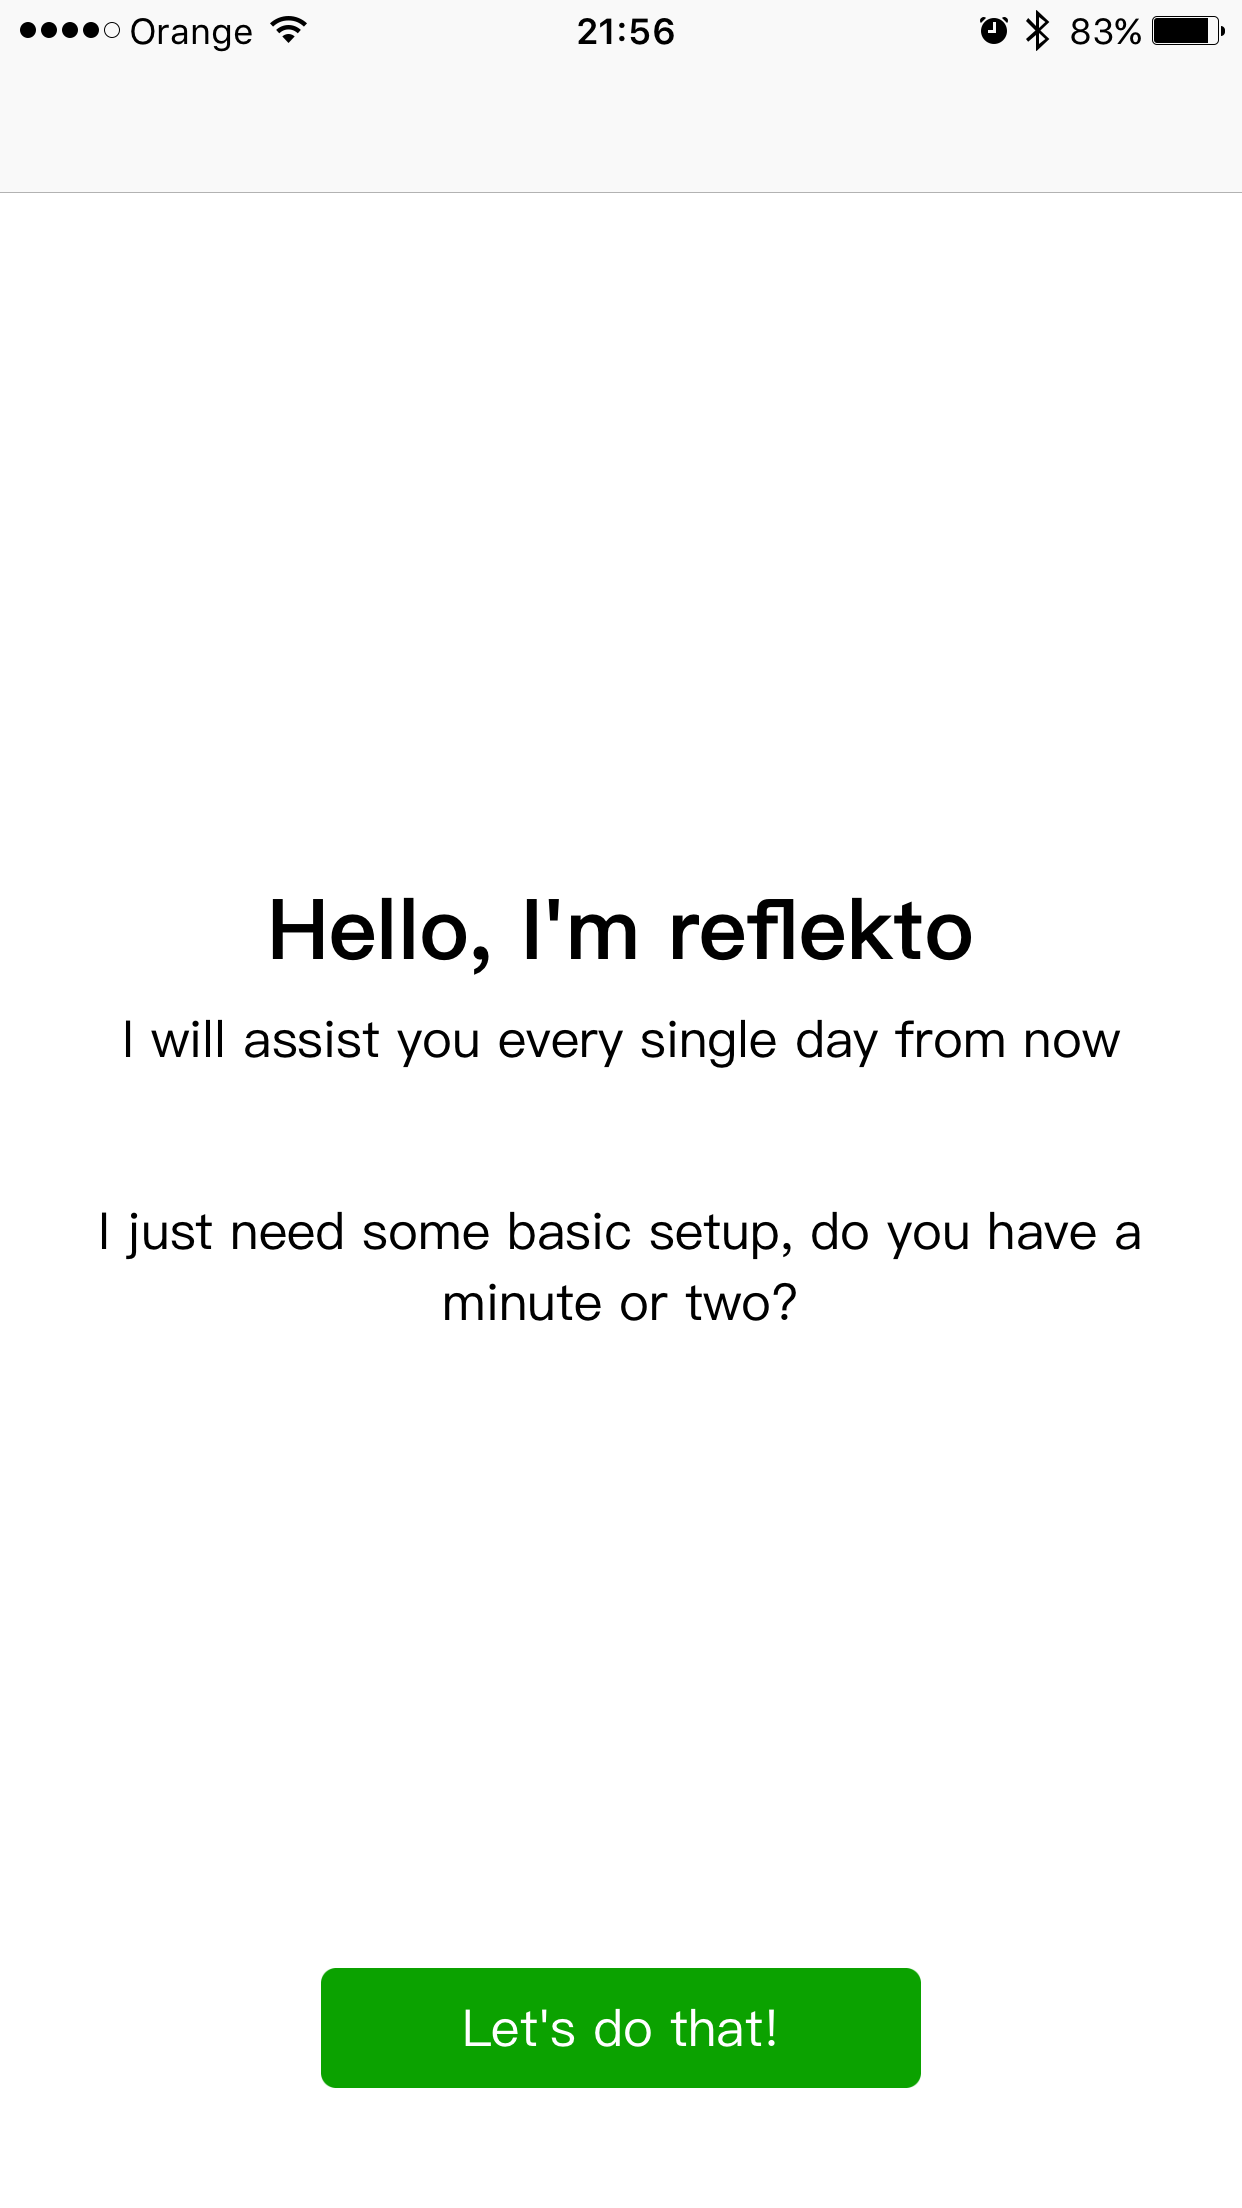
\includegraphics[width=0.4\textwidth]{ios-screens/setup1.png}
			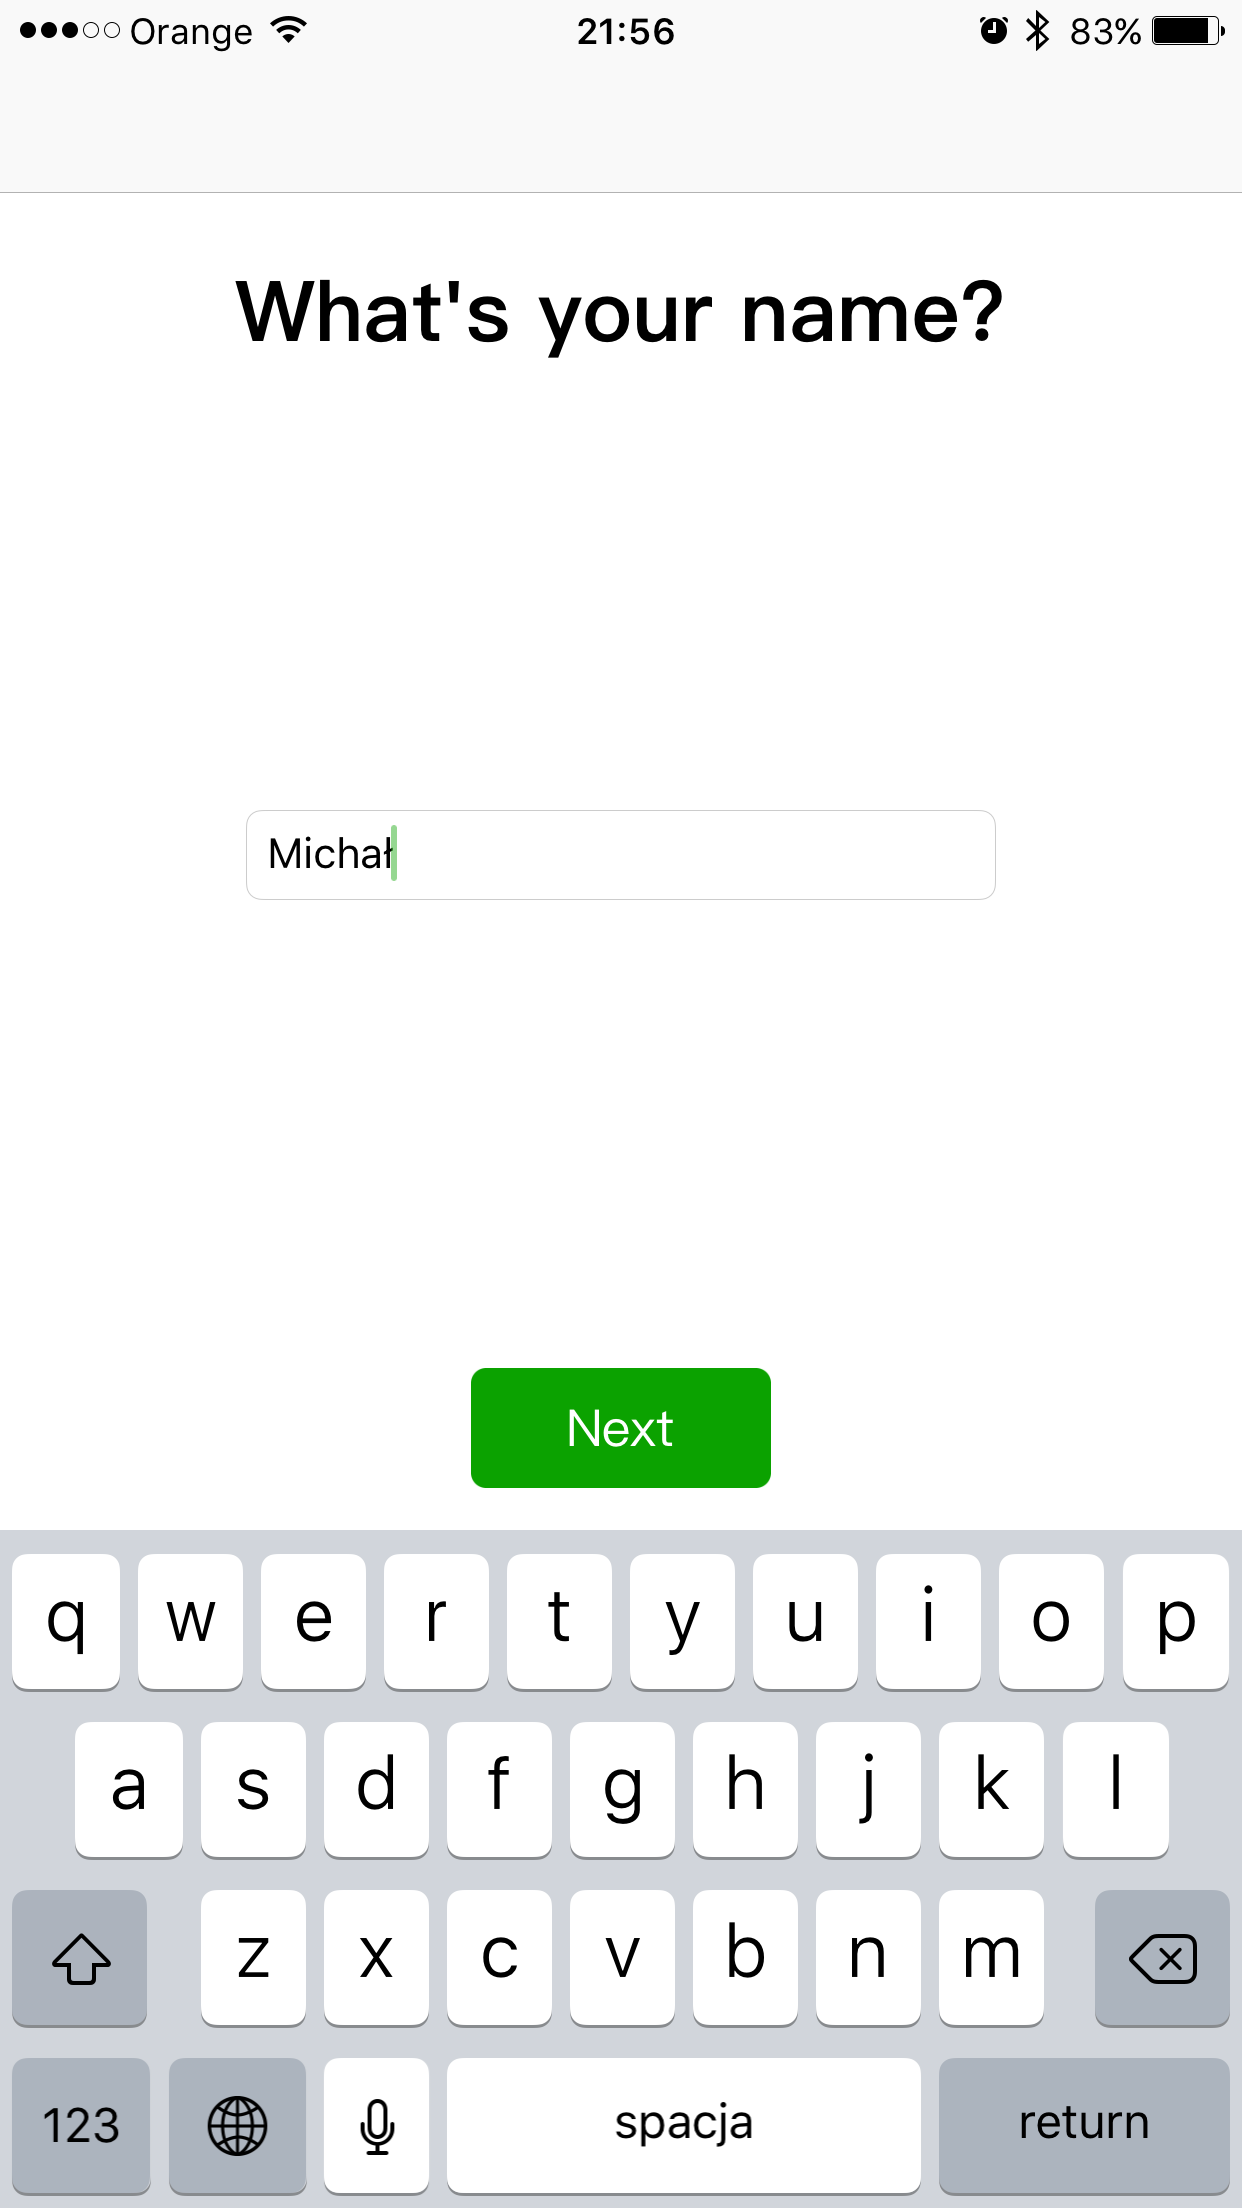
\includegraphics[width=0.4\textwidth]{ios-screens/setup2.png}
	}
		\caption {Wstęp do konfiguracji oraz pobranie imienia}
		\label{setup1}
	\end{figure}


	\newpage
	\item Kolejnym krokiem jest wybór płci. Dzięki jej znajomości generowany jest jeden z wielu komplementów na temat użytkownika lustra. (Rys. \ref{setup3})
	\begin{figure}[H]
	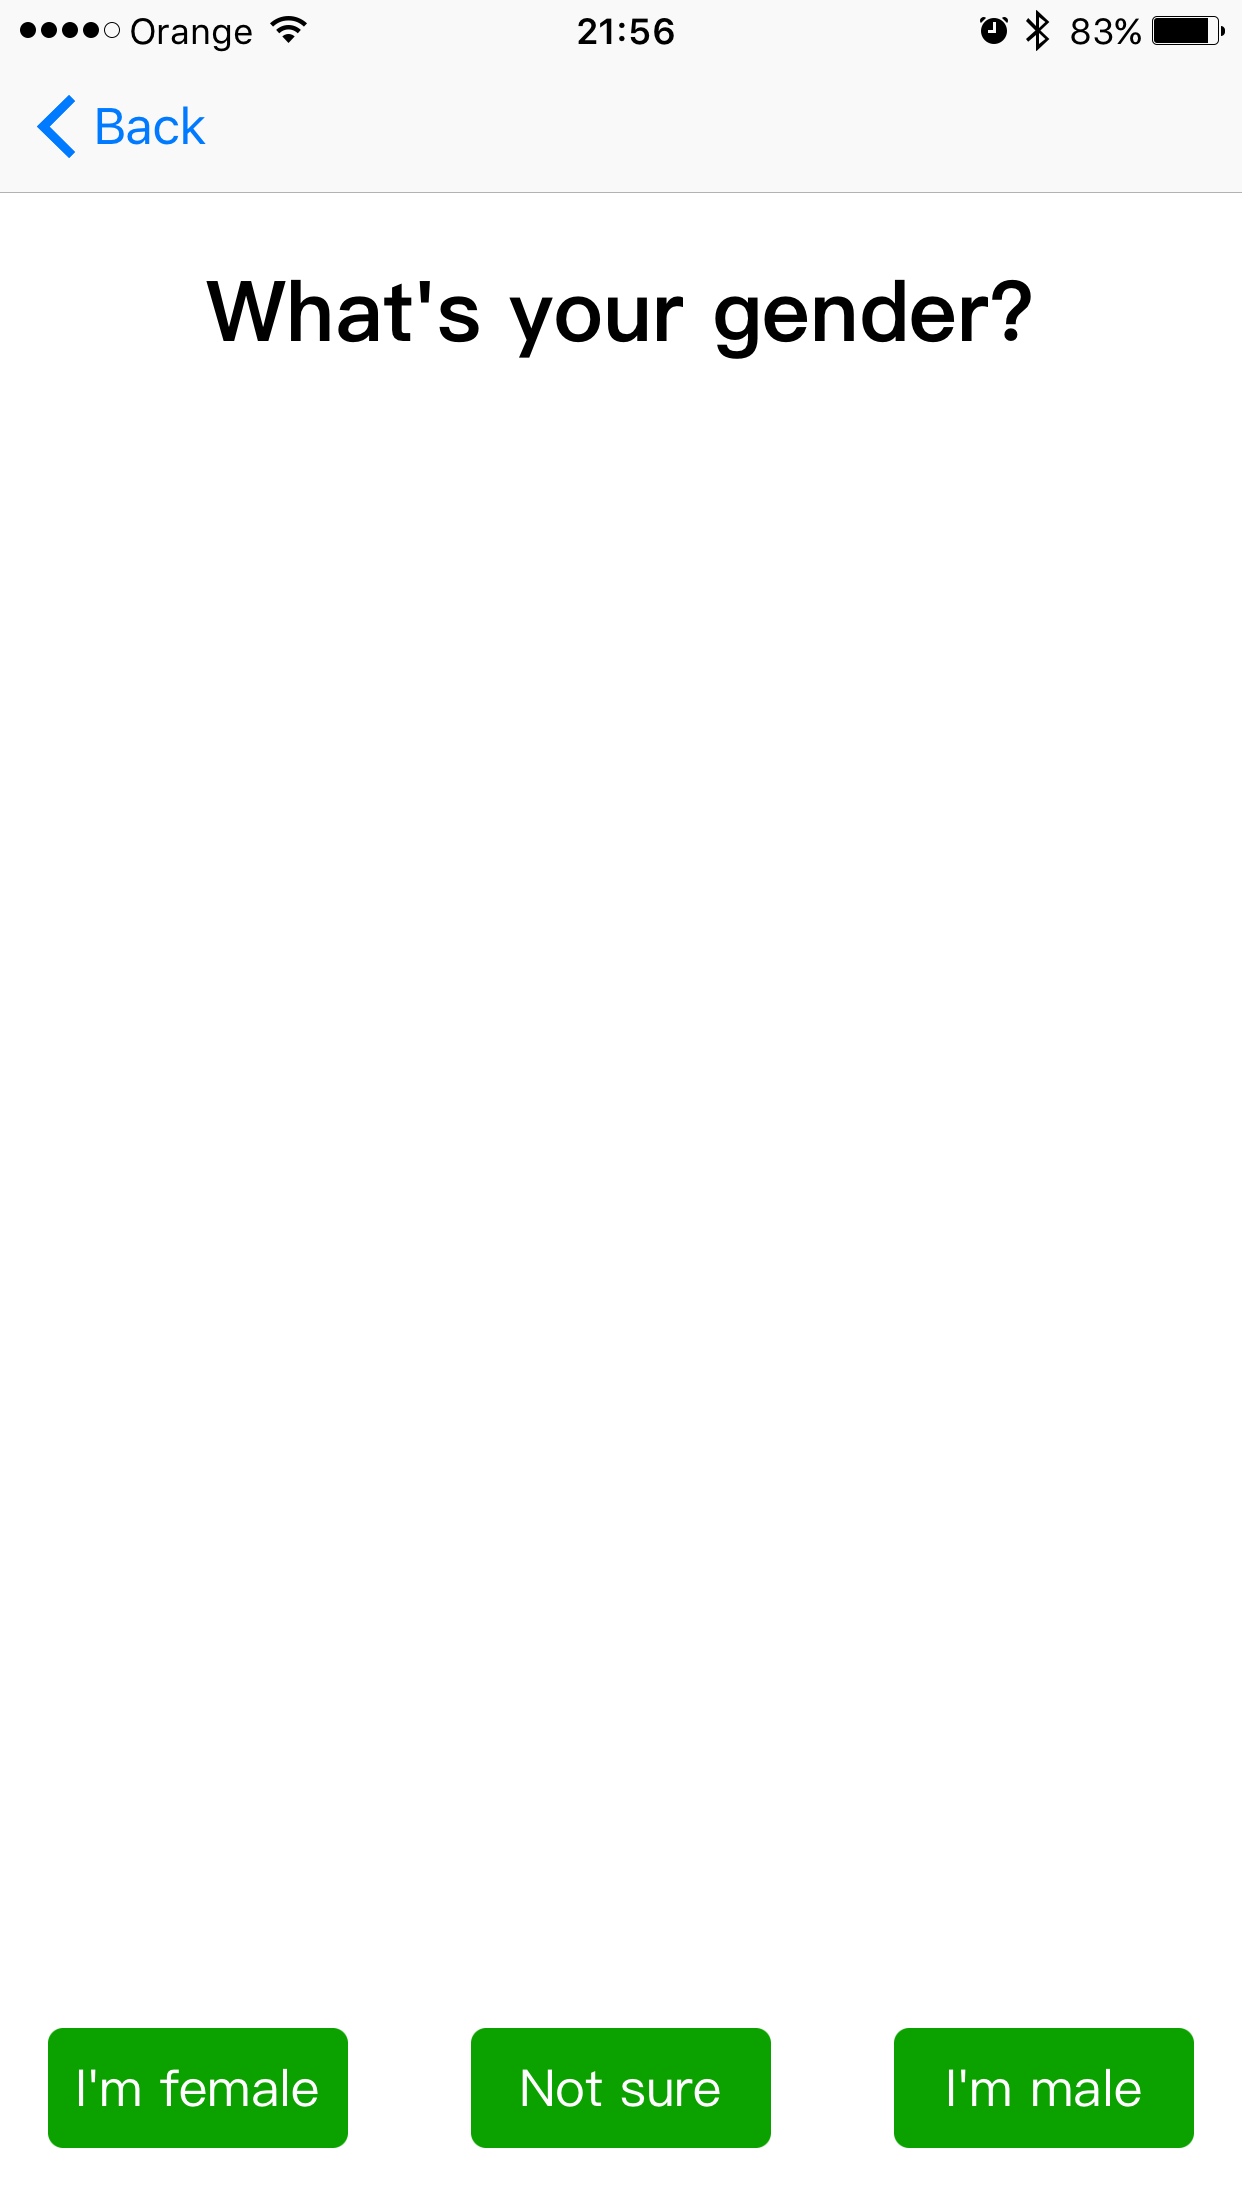
\includegraphics[width=0.5\textwidth,center]{ios-screens/setup3.png}
	\caption {Pobranie płci}
	\label{setup3}
	\end{figure}
\newpage
\item Czwarty ekran wyświetla trzy przyciski, dzięki którym użytkownik zezwala aplikacja na dostęp do określonych danych w swoim telefonie. Jest to niezbędny krok z powodu zabezpieczeń użytych w systemie iOS. Po przekazaniu wszystkich zgód ekran automatycznie przechodzi do kolejnego, nie ma potrzeby zatwierdzania. (Rys. \ref{setup4})
\begin{figure}[H]
	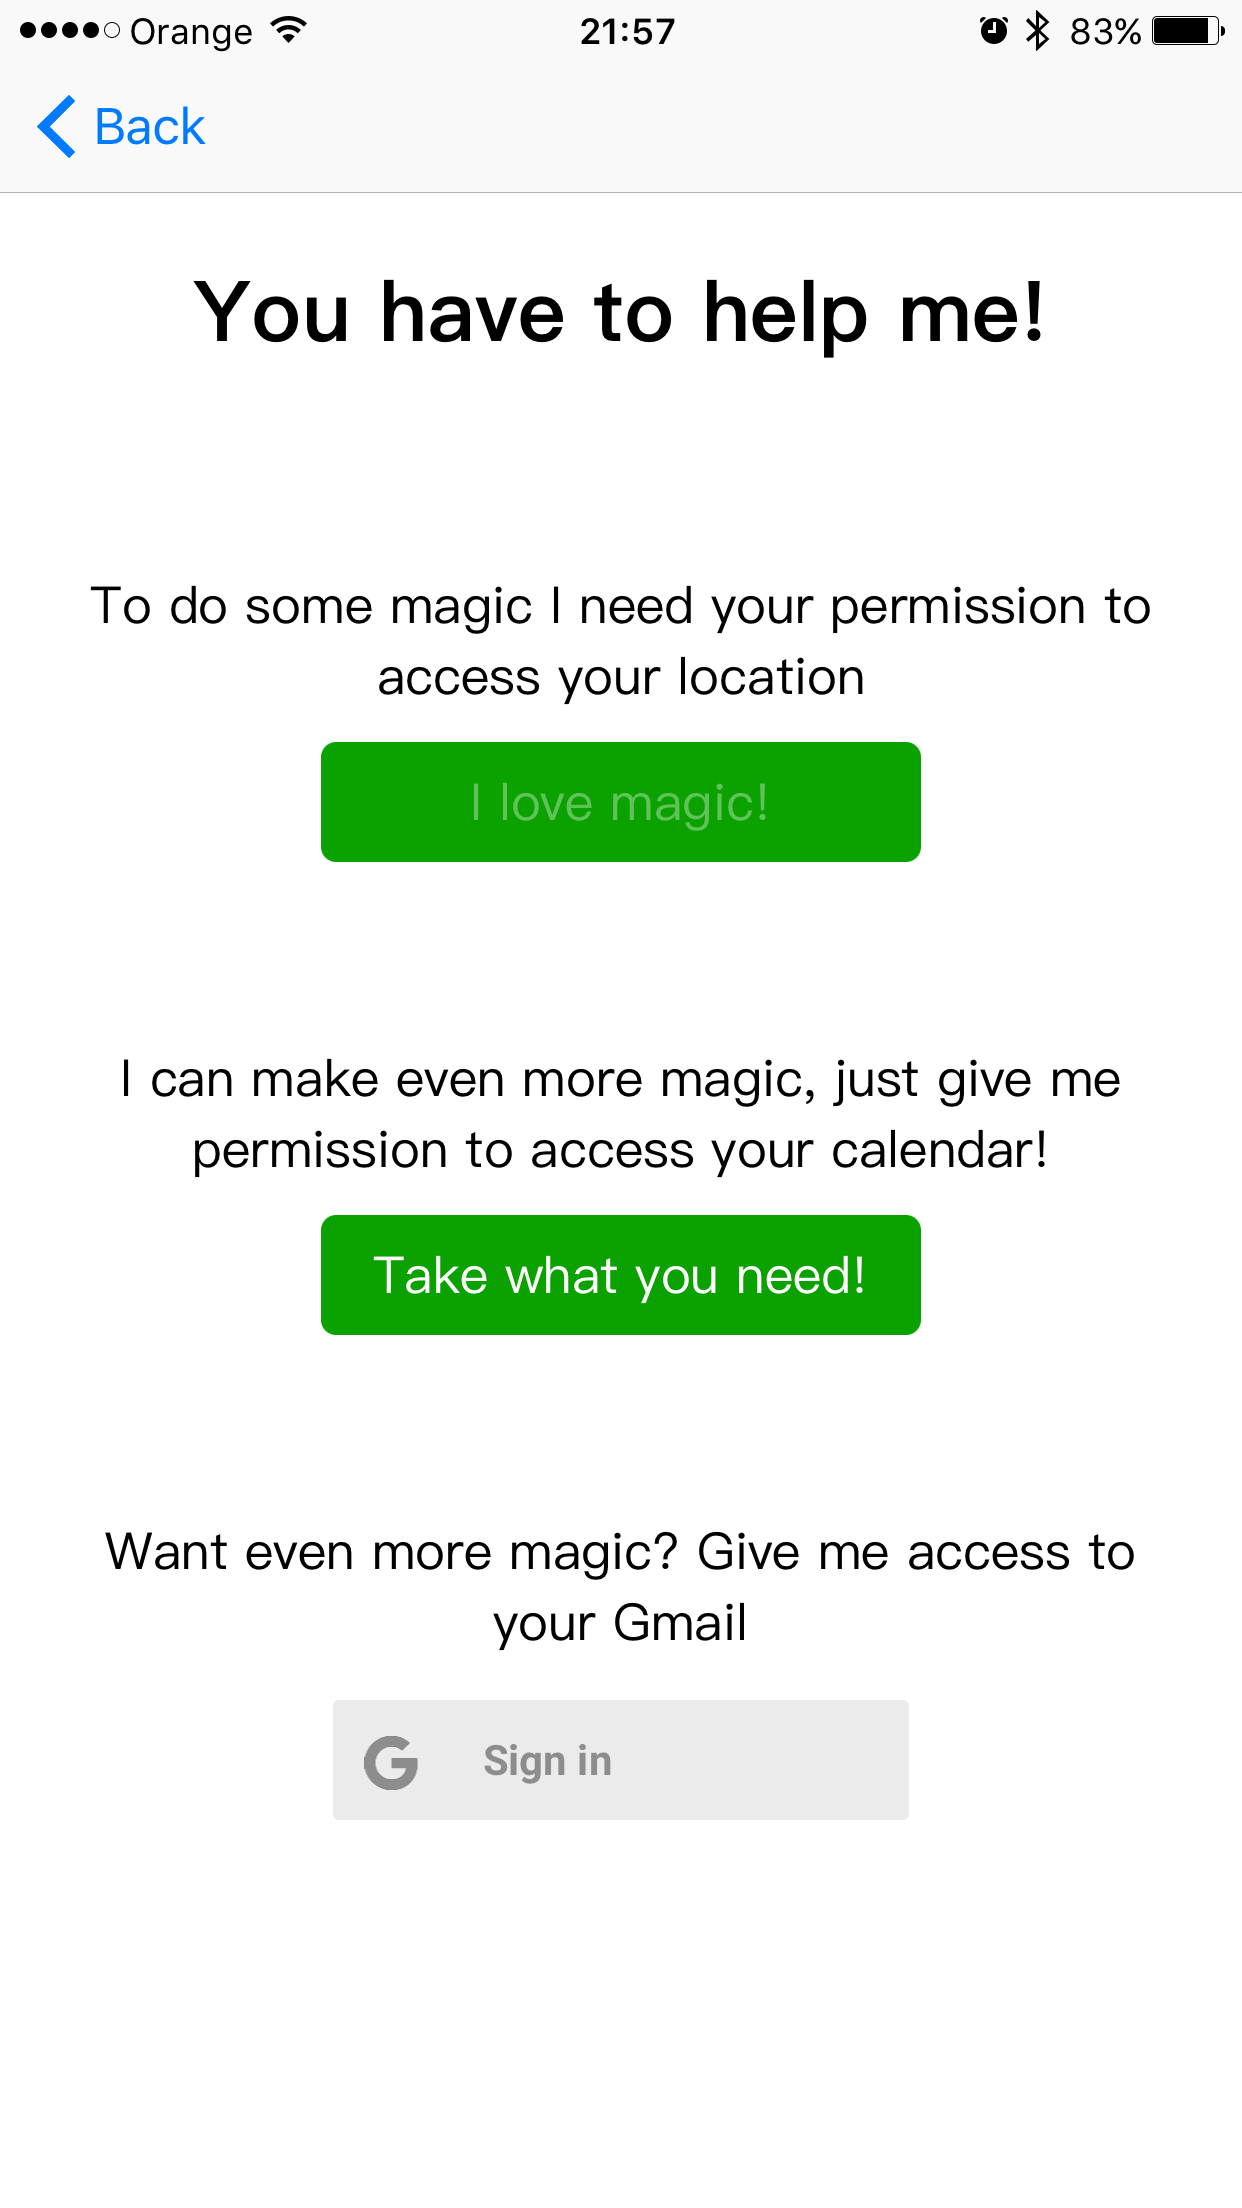
\includegraphics[width=0.5\textwidth,center]{ios-screens/setup4.png}
	\caption {Prośba o zezwolenia}
	\label{setup4}
\end{figure}
\newpage
\item Ostatnim krokiem jest wskazanie aplikacji miejsca zamieszkania oraz pracy. Użyta została do tego mapa, która ułatwia ten proces. Automatycznie po wejściu w ekran pobierana jest lokalizaja użytkownika i wskazywane jest aktualne miejsce, w którym się znajduje. (Rys. \ref{setup5})
\begin{figure}[H]
	\centerline{
	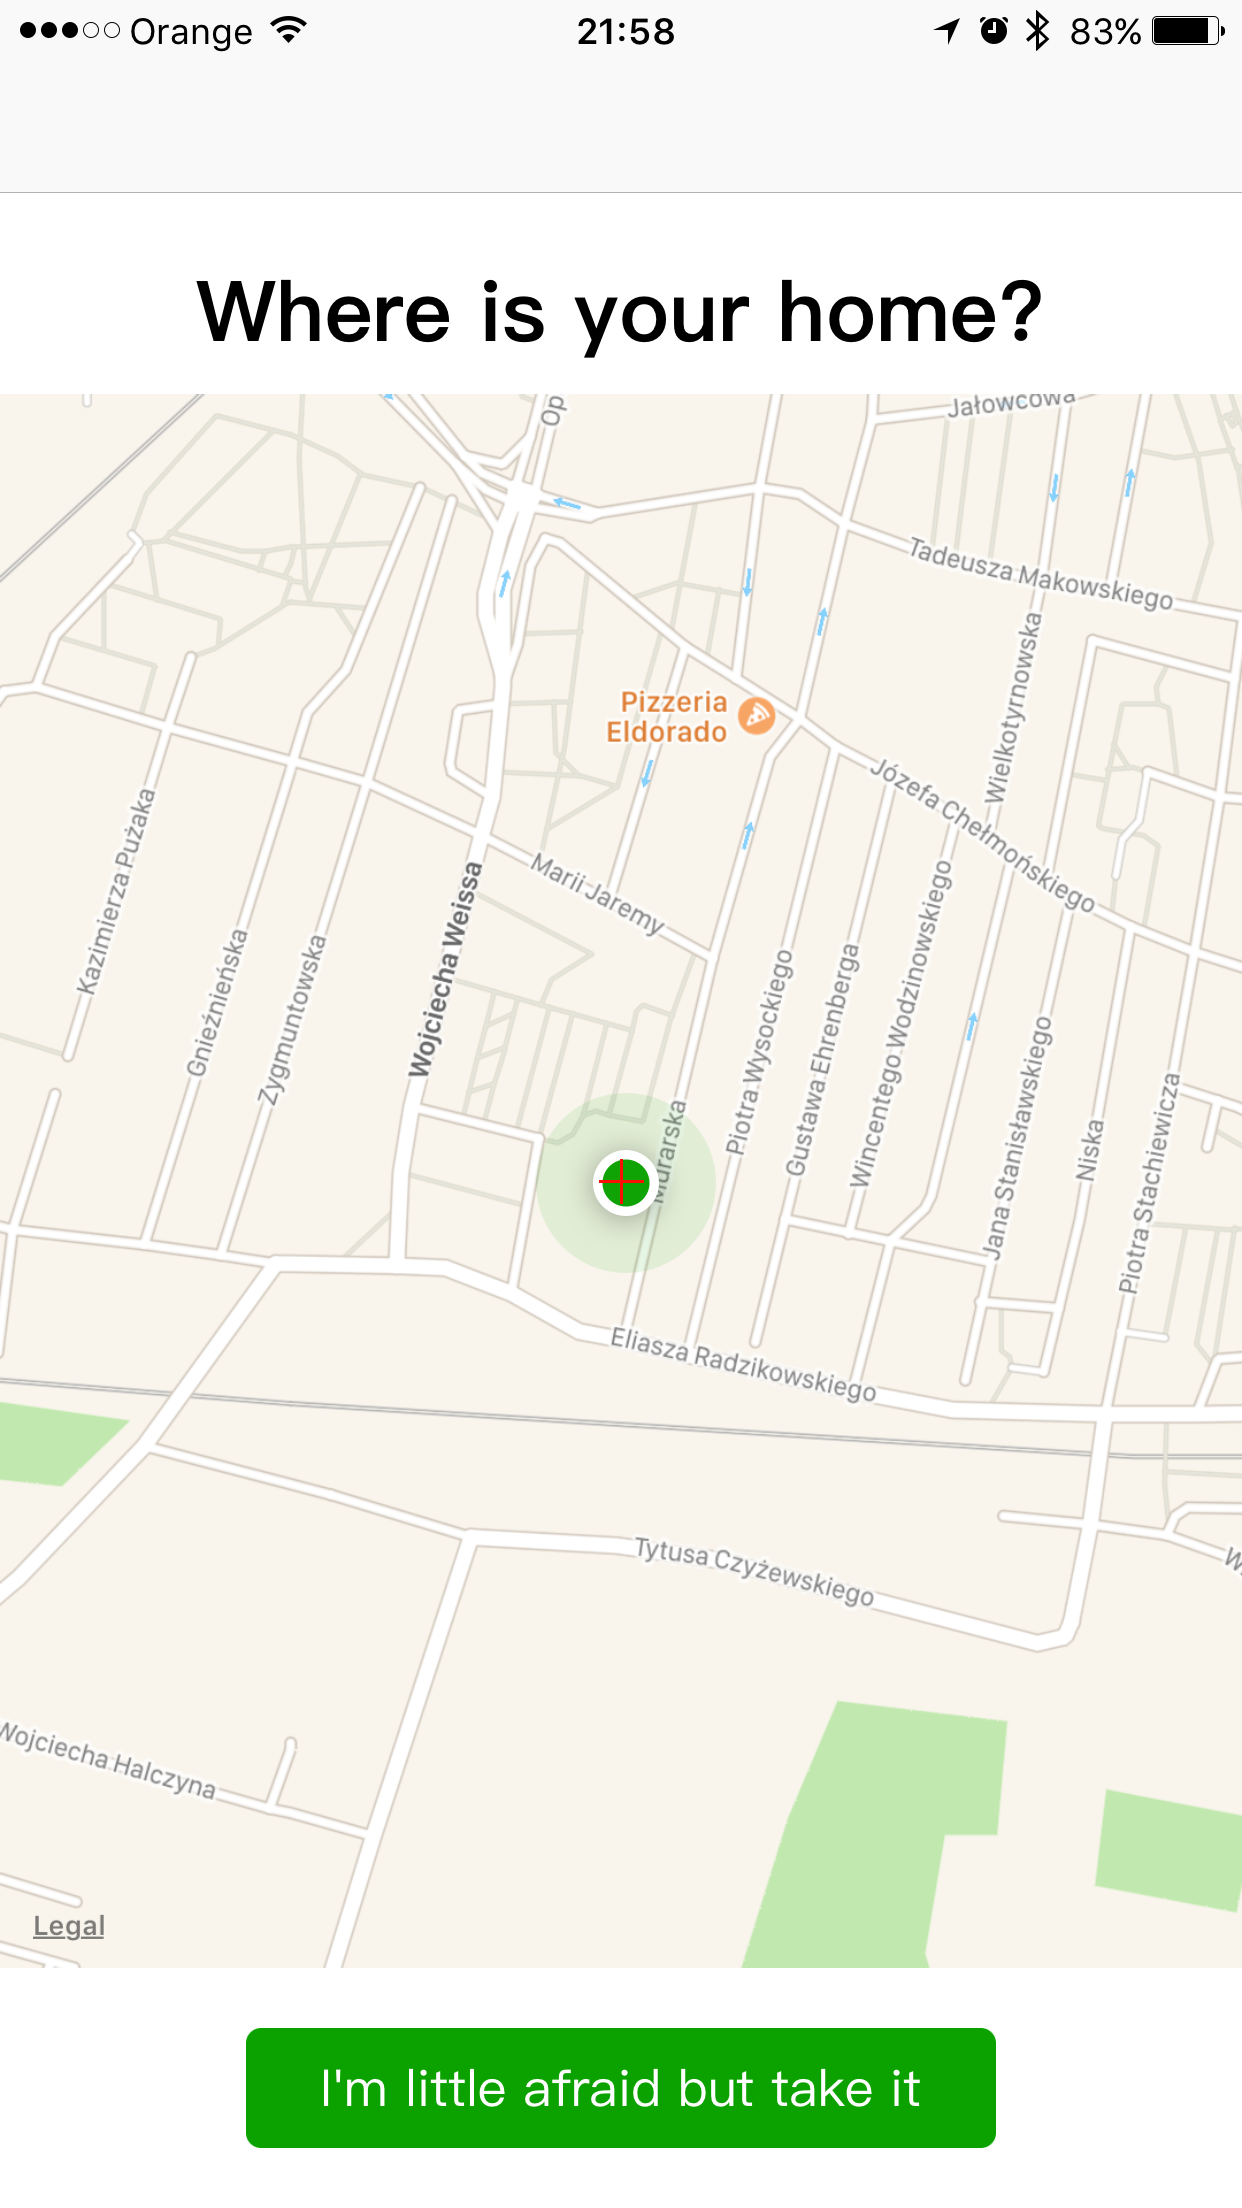
\includegraphics[width=0.4\textwidth]{ios-screens/setup5.png}
	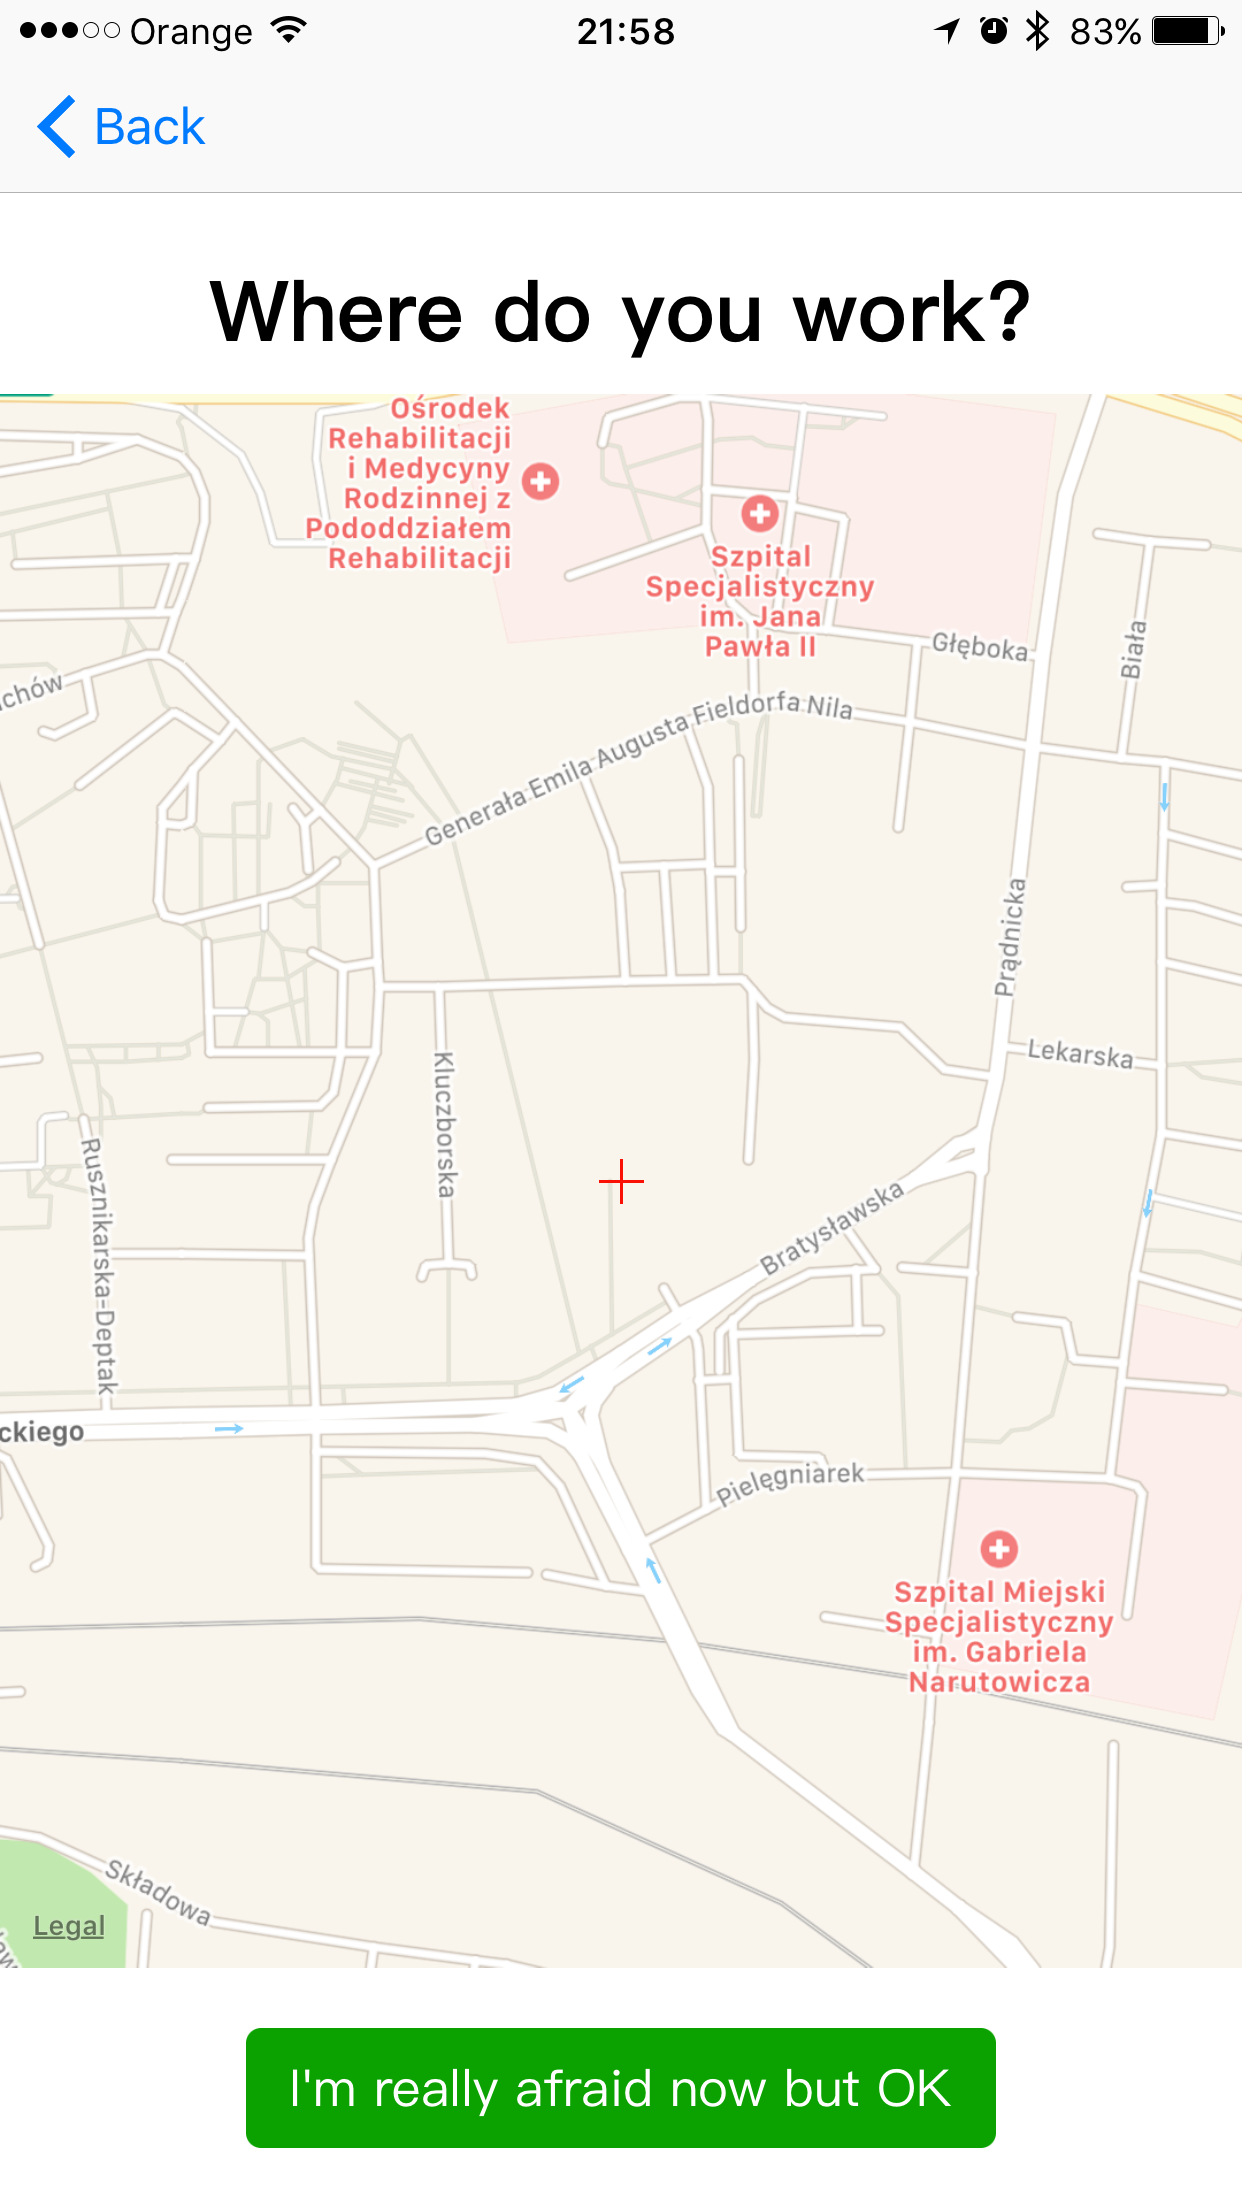
\includegraphics[width=0.4\textwidth]{ios-screens/setup6.png}
	}
	\caption {Wskazanie na mapie miejsce zamieszkania oraz miejsca pracy}
	\label{setup5}
\end{figure}
\newpage
\item Po wskazaniu miejsca zamieszkania i pracy aplikacja pokazuje ekran, w którym informuje o zakończeniu procesu konfiguracji. Naciśnięcie przycisku powoduje przejście do ekranu głównego. (Rys. \ref{setup7})
\begin{figure}[H]
	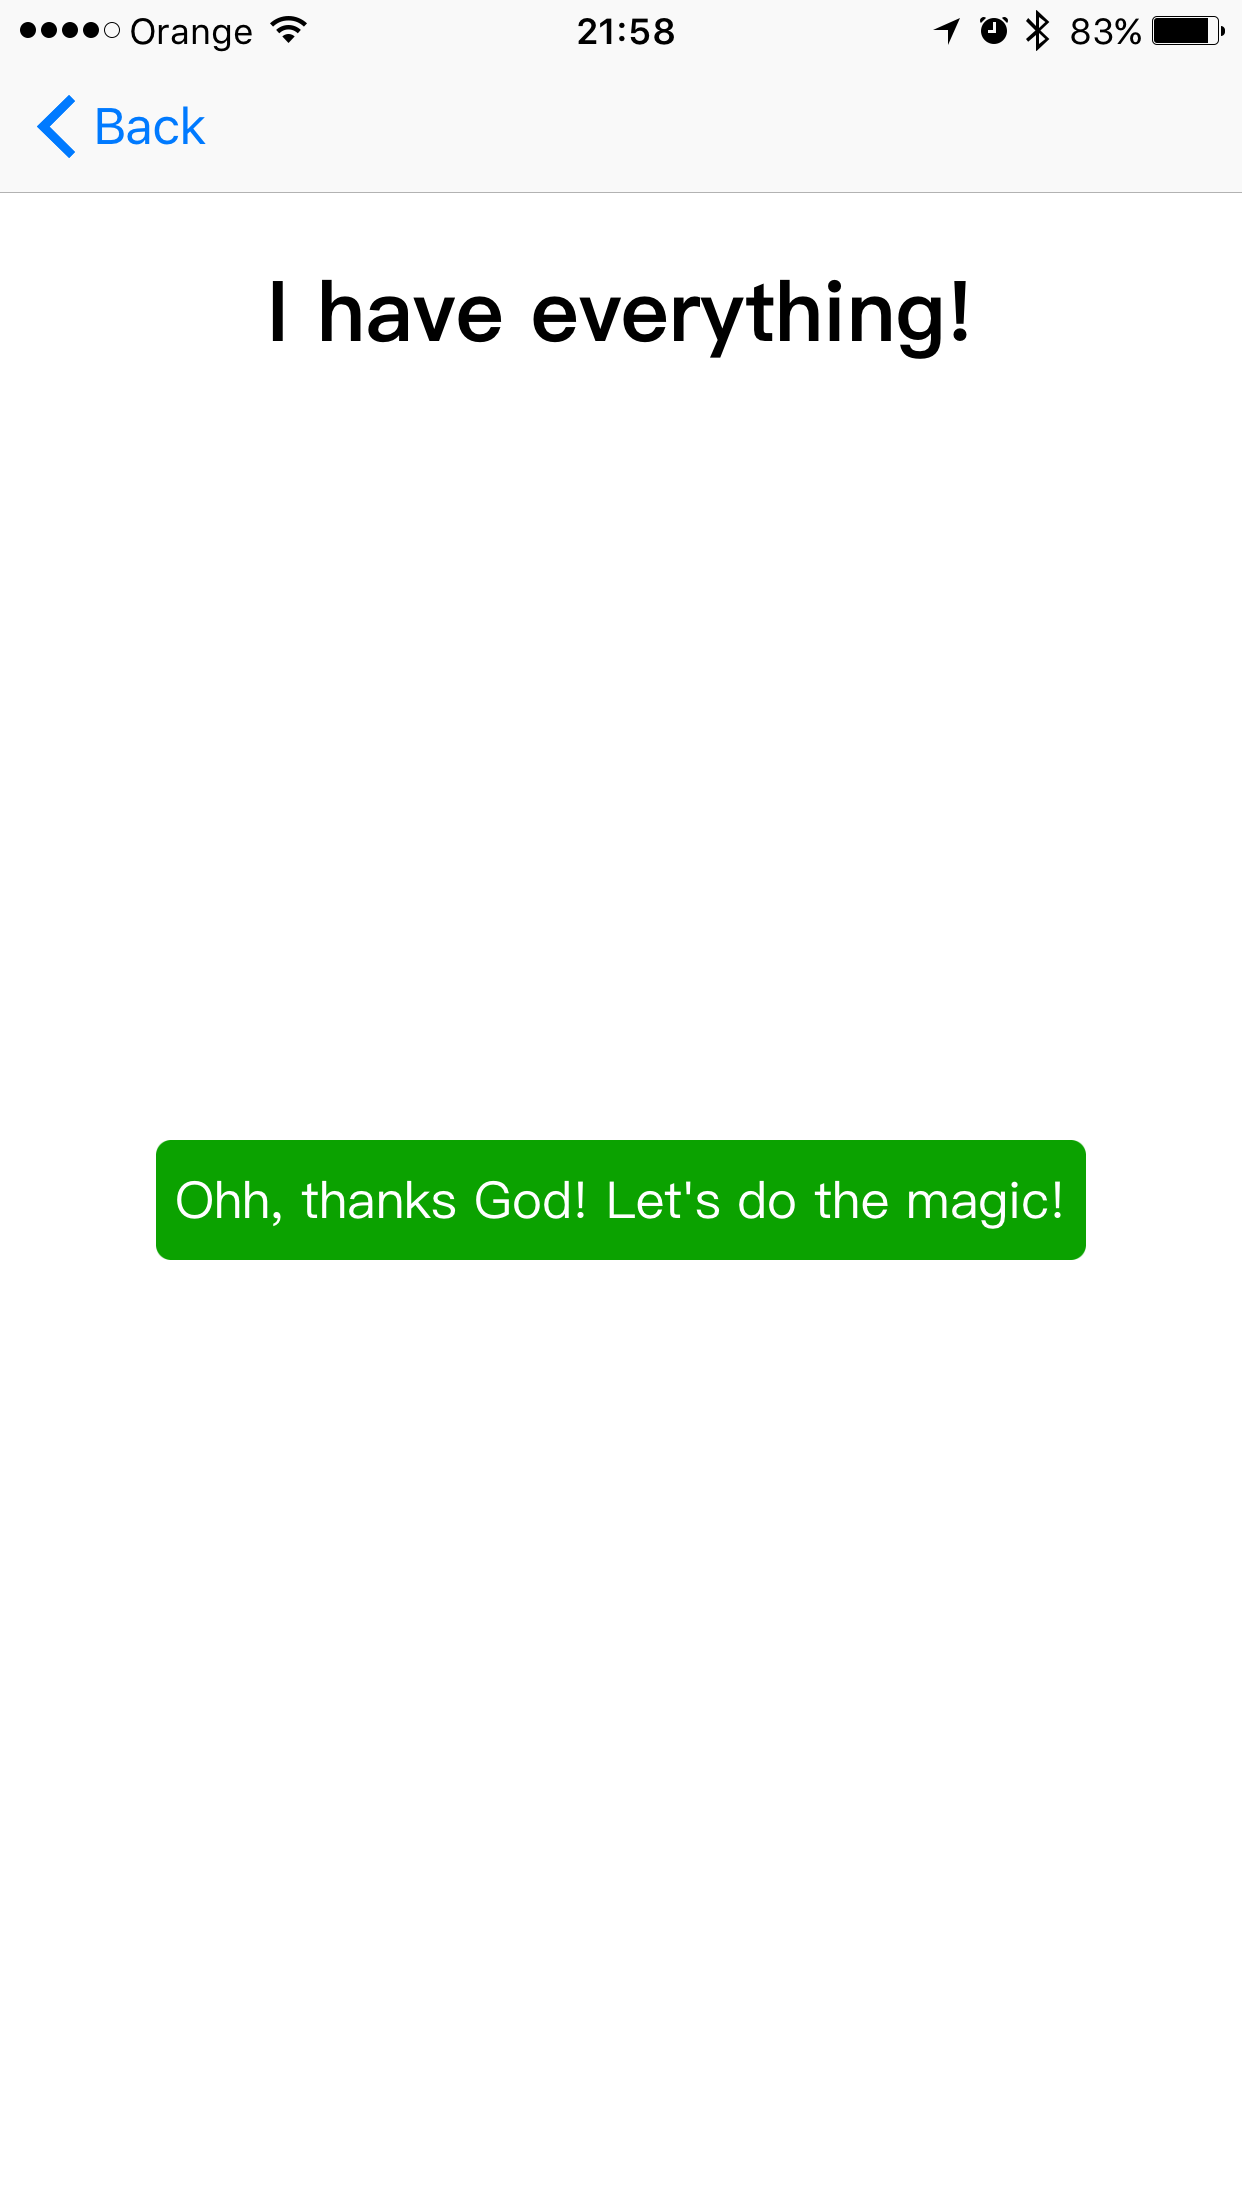
\includegraphics[width=0.5\textwidth,center]{ios-screens/setup7.png}
	\caption {Potwierdzenia zakończenia procesu konfiguracji}
	\label{setup7}
\end{figure}

\end{enumerate}

\newpage
\subsection{Ekran główny}
Po zakończeniu procesu konfiguracji lub każdorazowym późniejszym wejściu w aplikację użytkownikowi ukazuję się ekran główny (Rys. \ref{main_ios}). Znajdują się na nim przyciski do włączenia skanera Bluetooth, wyłączenia go oraz do przeprowadzenia procesu konfiguracji ponownie. Przyciski do włączania i wyłączania skanera są niezbędne, aby aplikacja przeszła review podczas umieszczania jej w sklepie AppStore. Po włączeniu skanera, można już wyjść z aplikacji lub zablokować ekran -- aplikacja będzie cały czas działała w tle.

\begin{figure}[H]
	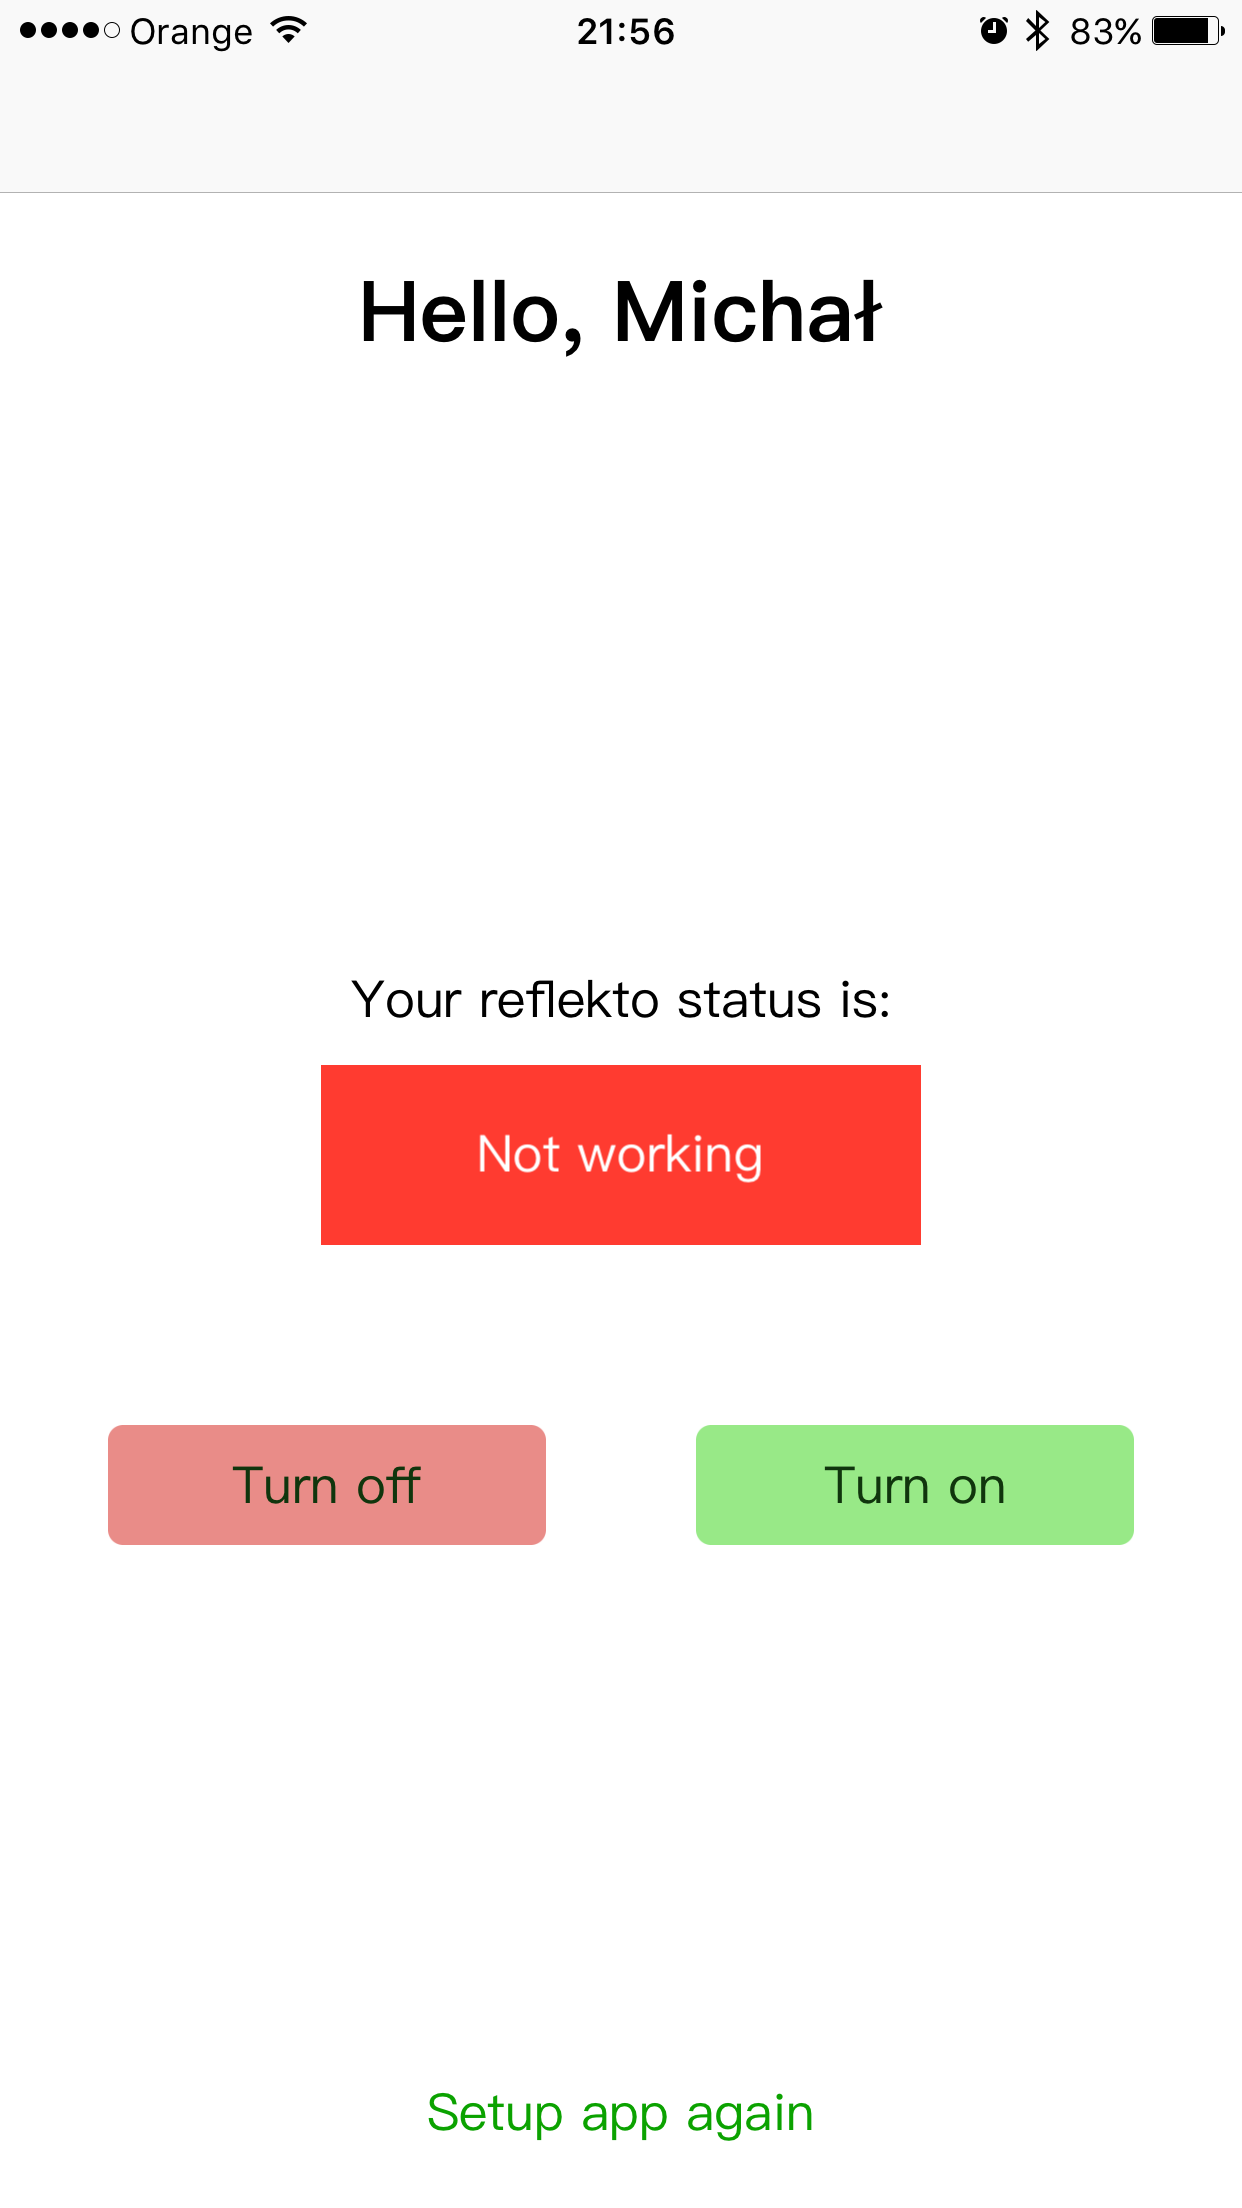
\includegraphics[width=0.5\textwidth,center]{ios-screens/main.png}
	\caption {Ekran główny}
	\label{main_ios}
\end{figure}

\subsection{Działanie w tle}
Z powodu bardzo restrykcyjnego podejścia systemu iOS do aplikacji działających w tle została ona maksymalnie zoptymalizowana, aby zużywała jak najmniej zasobów. Nadajnik Bluetooth w lustrze rozgłasza swoje pakiety z odpowienio niską mocą, aby połączenie odbywało się tylko wtedy, gdy lustro faktycznie jest w pobliżu telefonu. Dodatkowo Informacje pobierane z API są cachowane w celu optymalizacji zużycia energii. Po wykryciu nadajnika, aplikacja ma 10 sekund na połączenie się z lustrem oraz pobranie wszystkich danych. Aplikacja przed rozpoczęciem kolejnego skanowania oczekuje 4 sekundy po rozłączeniu, dzięki czemu powstaje okno czasowe, podczas którego kolejne urządzenie w zasięgu ma szansę na połączenie i wysłanie swoich informacji.

\subsection{Połączenie oraz problem długiego czasu rozłączania w iOS}
Po połączeniu z lustrem, aplikacja ma 2 sekundy na przesłanie odpowiedniego ciągu bajtów do charakterystyki konfiguracyjnej. Jeśli tego nie zrobi zostanie automatycznie rozłączona, a żadne dane przez nią przesłane nie zostaną wyświetlone na lustrze. Dodając do tego obniżoną moc nadajnika całkowicie zabezpiecza to możliwość nieautoryzowanego użycia lustra przez osoby trzecie. Znanym problem, który występuję w systemie iOS jest jego czas rozłączania się z urządzeniem. Po wydaniu komendy rozłączenia nie jest to robione natychmiastowo, lecz dopiero po około 7 sekundach. Rozwiązaliśmy ten problem wpisaniem do charakterystyki konfiguracyjnej odpowiedniego ciągu bajtów, który zaraz po ich otrzymaniu rozłącza urządzenie. Rozłącznie po stronie sprzętu realizowane jest natychmiast, stąd nie występuje problem długiego rozłączania.

\subsection{Programowanie funkcyjne}
Aplikacja pobiera dane asynchronicznie, jest to wykonane w kodzie w bardzo schludny sposób dzięki zastosowaniu programowania funkcyjnego. Wykonane zostało to z użyciem biblioteki RxSwift. Poniżej fragment kodu ilustrujący, jak łatwo połączyć kilka różnych informacji pobieranych asynchroniczne w jeden element, który można przesłać do urządzenia. Reactive Functional Programming to w ostatnich czasach bardzo popularne i pożadne podejście podczas programowania aplikacji pobilnych.

\begin{lstlisting}
Observable.zip(
	 DataManager.timestamp,
	 DataManager.weather,
	 DataManager.nextEvent, 
	 DataManager.name,
	 DataManager.greeting, 
	 DataManager.compliment, 
	 DataManager.unreadMailsCount, 
	 DataManager.travelToWorkTime)
	  	.subscribe(onNext: { [weak self] 
	  						(timestamp, weather, nextEvent, name, greeting,
	  						compliment, unreadMailsCount, travelWorkTime) in
	  							//wyslanie danych do lustra
\end{lstlisting}

\subsection{Pobierane dane i sposób ich pobrania}

\begin{itemize}
	\item Godzina
	\item Miejsce, pogoda -- na podstawie wyznaczonej lokalizacji telefon wysyła zapytanie do Dark Sky API podając w parametrze m. in. długość oraz szerokość geograficzną. Otrzymany w odpowiedzi JSON parsowany jest na obiekt, z którego później wybierana jest temperatura. Miejsce wyznaczone jest również na podstawie szerokości i długości geograficznej używając wbudowanego  API Apple Maps.
	\item Wiatr -- pobierana z Dark Sky API
	\item Pogoda - dodatkowa informacja. -- pobierana z Dark Sky API
	\item Powitanie
	\item Imię
	\item Komplement
	\item Czas dojazdu do pracy -- wyznaczany na podstawie prawdziwego ruchu na ulicach w aktualnym momencie
	\item Ilość nieodczytanych mail
	\item Następne wydarzenie w kalendarzu
	
\end{itemize}

\subsection{Testy jednostkowe}
Jednym z trudniejszych algorytmów zastsowanych w aplikacji jest algorytm podziału danych na paczki. Z tego powodu zostały napisane do niego testy jednostkowe a sam algorytm powstał dzięki TDD (Test Driven Development)

\section{Sposób replikacji}

\subsection{iOS}
Po sklonowaniu repozytorium z brancha master, należy w konsoli przejść do folderu z projektem oraz uruchomić komendę 
\begin{lstlisting}
pod install
\end{lstlisting}
Jeśli komenda nie jest dostępna należy zainstalować oprogramowanie CocoaPods

\subsection{nRF 52}
Najprostszym sposobem umieszczenia oprogramowania na DevKicie nRF52 jest skopiowanie pliku \textit{nRF\_Reflekto.hex} do urządzenia J-LINK wyświetlonego przez komputer. Folder z wygenerowanymi plikami został specjalnie pozostawiony w repozytorium: \begin{lstlisting}
/reflekto-embedded/nRF_Reflekto_Services/Output/nrf52832_xxaa/Exe/
\end{lstlisting} 
Wymagane jest wcześniejsze posiadanie zainstalowanego SoftDevice na płytce. Można tego dokonać poprzez apliakcję nRFgo Studio. Aplikacja była rozwijana i testowana z użyciem SoftDevice
\begin{lstlisting}
s132_nrf52_4.0.2_softdevice.hex
\end{lstlisting}
Inną możliwością jest własnoręczne skompilowanie plików źródłowych. Projekt rozwijany był z użyciem IDE Segger Embedded Studio 3.12. Po pobraniu repozytorium wystarczy uruchomić plik projektu
\textit{nRF\_Reflekto.emProject }i wybrać z menu \textit{Build/Build and run}. Dodatkowo z użyciem tego programu mamy możliwość podłączenia debuggera korzystającego z RTT i otrzymanie logów podczas pracy urządzenia.

\section{Podsumowanie}
Projekt rozwijany był z użyciem systemu kontroli wersji GitHub. Wszystkie postępy prac dostępne są pod adresem: \url{https://github.com/Solstico}
	
	
\end{document}